\documentclass[10pt,a4paper]{article}
\usepackage[utf8x]{inputenc}
\usepackage{ucs}
\usepackage{amsmath}
\usepackage{amsfonts}
\usepackage{amssymb}
\usepackage{hyperref}
\usepackage{pgf, tikz}

\title{\textbf{Rendering Aurora}}
\author{
	Tao, Du\\
	\texttt{taodu@stanford.edu}
	\and
	Wenlong, Lu\\
	\texttt{wenlongl@stanford.edu}
}
\date{\today}

\begin{document}

\maketitle

\section{Introduction}

\begin{figure}[h]
\centering
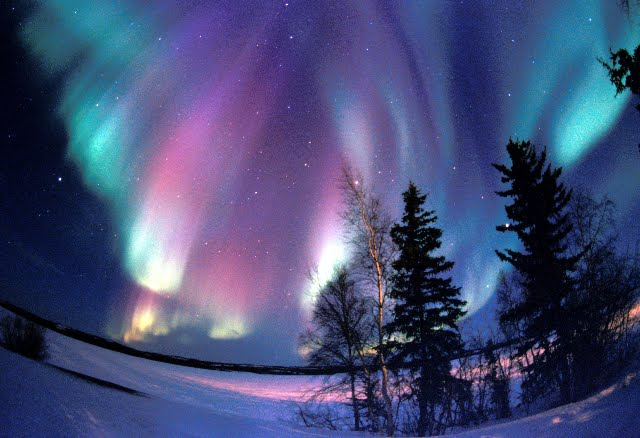
\includegraphics[width=0.7\linewidth]{./reference}
\caption{an aurora image from Tessa Macintosh, 2006}
\label{fig:reference}
\end{figure}

Aurora is a splendid natural phenomenon which has not been fully understood by human beings yet. As a result, rendering a physically plausible aurora remains to be challenging. In our final project, we provide a complete pipeline to render aurora based on physical simulation and volumetric rendering. The aurora shape is generated by simulating a 2D footprint, then a volume grid is built based on the ddensity of the footprint. We generate photons inside the volume for volumetric photon mapping. The rendering result is also enhanced by applying multiple kinds of noises and customized colormap.

The remaining sections are organized as follows: section 2 covers all the algorithms and technical details in rendering aurora; section 3 gives the final image; The challenges and division of work are provided in section 5.

\section{Algorithms and Techniques}

\subsection{Creating the Footprint}

To create a footprint that can give a natural looking outline for the 
aurora, we used a simple 2D fluid simulation as suggested in \cite{lawlor2011interactive}.
Different from what they did in the original paper, we initialize the 
density field and the velocity field with sine wave functions, shown in 
Figure \ref{fig:foorprint}(left). And we ran the simulation for a few frame to get a footprint 
on a straight line (middle). Then we use a low frequency noise curve to remap 
the density field and create our final foorprint (right).

\begin{figure}[h]
\centering
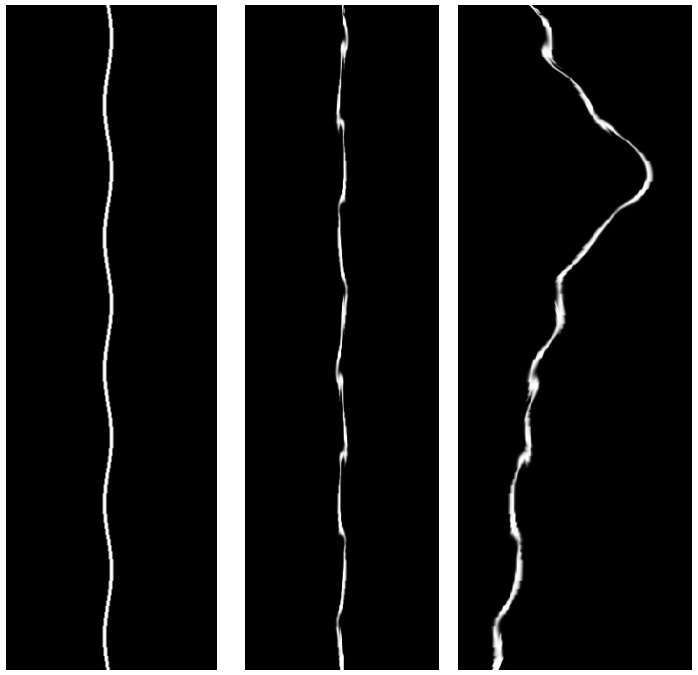
\includegraphics[width=0.7\linewidth]{./footprint}
\caption{Footprint}
\label{fig:foorprint}
\end{figure}


\subsection{Generate photons}

After creating the footprint, the next thing is to build an axis-aligned bounding box as the volume that contains the aurora. We divided the box into small grids, and the density in each grid is computed from the footprint. The density here is used to decide whether a point is inside aurora or not.

Besides the aurora density above, we also included the air density in our volume. The air density decreases exponentially along the height, and is used to modulate the absorption and scattering parameters at different points.

We followed the method suggested in \cite{baranoski2000simulating} to generate photons inside the volume. We first traced multiple electron beams from uniformly distributed starting points in the volume. For each beam, the electron can collide with the atoms in the atmosphere and therefore be deflected. We simulated this process and generated photons at each deflection point in the beam. Specifically, for each starting point $\mathbf{p}$, we first move the electron along the geomagnetic vector $\mathbf{B}$, whose distance is determined by a random step $s$, then we add some displacement in the plane perpendicular to the geomagnetic vector according to a uniformly sampled angle $\beta$:

\[
\mathbf{p}_{new} = \mathbf{p} + s\mathbf{B} + t\mathbf{u}\cos(\beta) + t\mathbf{v}\sin(\beta)
\]

where $\mathbf{u}$, $\mathbf{v}$ and $\mathbf{B}$ form a Cartesian coordinate system. The parameter $t$ determines how much the electron deviates from the geomagnetic vector. We compute $t$ by sampling in the angle $\alpha$ between $\mathbf{p}_{new} - \mathbf{p}$ and $\mathbf{B}$:

\[
\tan{\alpha} = \frac{t}{s}
\]

and $\alpha$ is uniformly sampled between $\alpha_D$ and $\alpha_D - \Delta \alpha$. We iterate this procedure multiple times to generate hundreds of deflection points along the electron beam, and we place a photon at each deflection point. The radiance of the photon is interpolated from a pre-defined color map. Instead of applying the color map in \cite{baranoski2000simulating}, we built up our own color maps for better visual effects.

\begin{figure}[h]
\centering
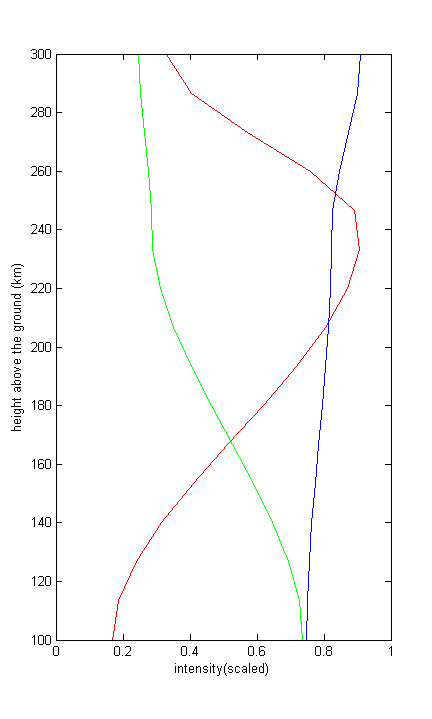
\includegraphics[width=0.5\linewidth]{./colormap}
\caption{customized colormap}
\label{fig:colormap}
\end{figure}

\subsection{Volumetric photon mapping}

Unlike the paper \cite{baranoski2000simulating} which did rendering based on rasterizing photons into image films directly, we used volumetric photon mapping to render the final images. For each point inside the volume, we used the photons nearby to compute \texttt{Lve}, the radiance of the emissive/in-scattering light at that specific point. The radiance comes from the weighted sum of all the photons inside a ball around the point with a predefined radius $r$, where the weight is computed from a Gaussian kernel.

Both photon generating and volumetric photon mapping are implemented in a custom class \texttt{AuroraDensity}, which is inherited from \texttt{VolumeRegion} in pbrt.

\subsection{Adding Noise}

During the process of generating photons and searching photons, we added 
multiple 1D and 2D perlin noises to make our aurora more visually interesting.

\begin{enumerate}
    \item A high frequncy, small magnitude 1D noise is used to perturb 
    the starting height where we generate the electrons.
    \item A low frequncy, large magnitude 1D noise is used to perturb 
    the height of the photon when we lookup the color (not intensity).
    \item A medium frequncy, medium magnitude 2D noise is used to 
    perturb the radius we use to search for photon. So the density of 
    aurora curtain varies. 
\end{enumerate}

The effect is illustrated in the Figure \ref{fig:noise} below.
\begin{figure}[h]
\centering
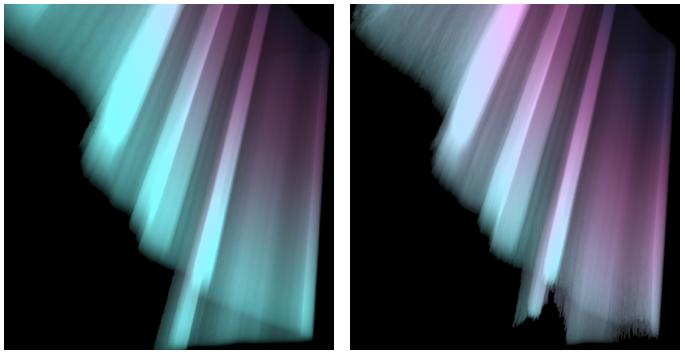
\includegraphics[width=0.8\linewidth]{./noise}
\caption{Adding Noise}
\label{fig:noise}
\end{figure}

\subsection{Tracing the Shadow Ray}

\begin{figure}[h]
\centering
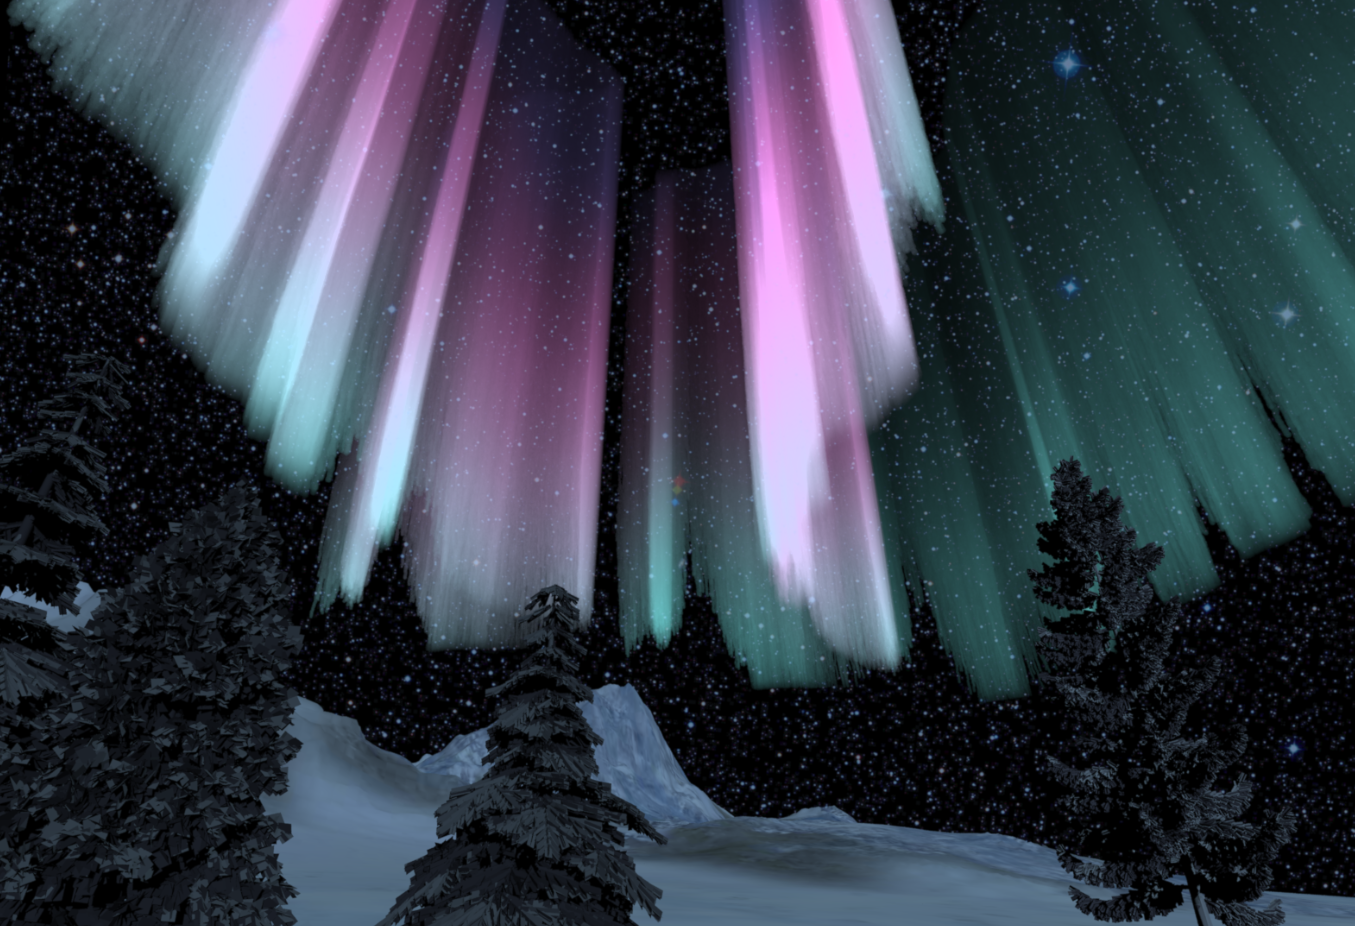
\includegraphics[width=0.7\linewidth]{./no_light_cast}
\caption{aurora: no cast light on the mountain}
\label{fig:no_light_cast}
\end{figure}

Since aurora is emitting light in the scene, we expect there should be light cast on the other objects if there is not occlusion between them. However, when we tried it with the default\texttt{SamplerRenderer}\ and \texttt{DirectLightingIntegrator} in pbrt, it turned out that they only took absorption and out scattering into consideration when tracing a shadow ray in the scene. As we don't have any other strong light source in the scene, it is not surprising all the shadow rays are very dim, and attenuated further by transmitting the volume.

As a result, we extent the \texttt{Renderer} by adding a new function \texttt{Emission}. It wraps the underlining volumeIntegrator and calls its \texttt{Li} function. For each shadow ray, given the radiance $\mathbf{Li}$ from the surface integrator, we compute the emission/in-scattering results $\mathbf{Lvi}$ and the transmittance $\mathbf{T}$. The final radiance $\mathbf{L}$ is defined as

\[
\mathbf{L = T * Li + Lvi}
\]

Adding this function in the renderer will instantly render the aurora light cast on other objects in the scene, as can be seen from Figure \ref{fig:no_light_cast} and Figure \ref{fig:aurora} below.

\section{Results}

The final scene includes a landscape model, three different tree models, three aurora sheets and a background texture. Each aurora sheet is generated by simulating a footprint described in section 2.1. The light cast on the mountain is enhanced explicitly in the program when we trace the shadow ray along the volume. All the pbrt scrips, models and source codes can be found in \href{https://github.com/dut09/pbrt-v2}{our github site}. 

\begin{figure}[h]
\centering
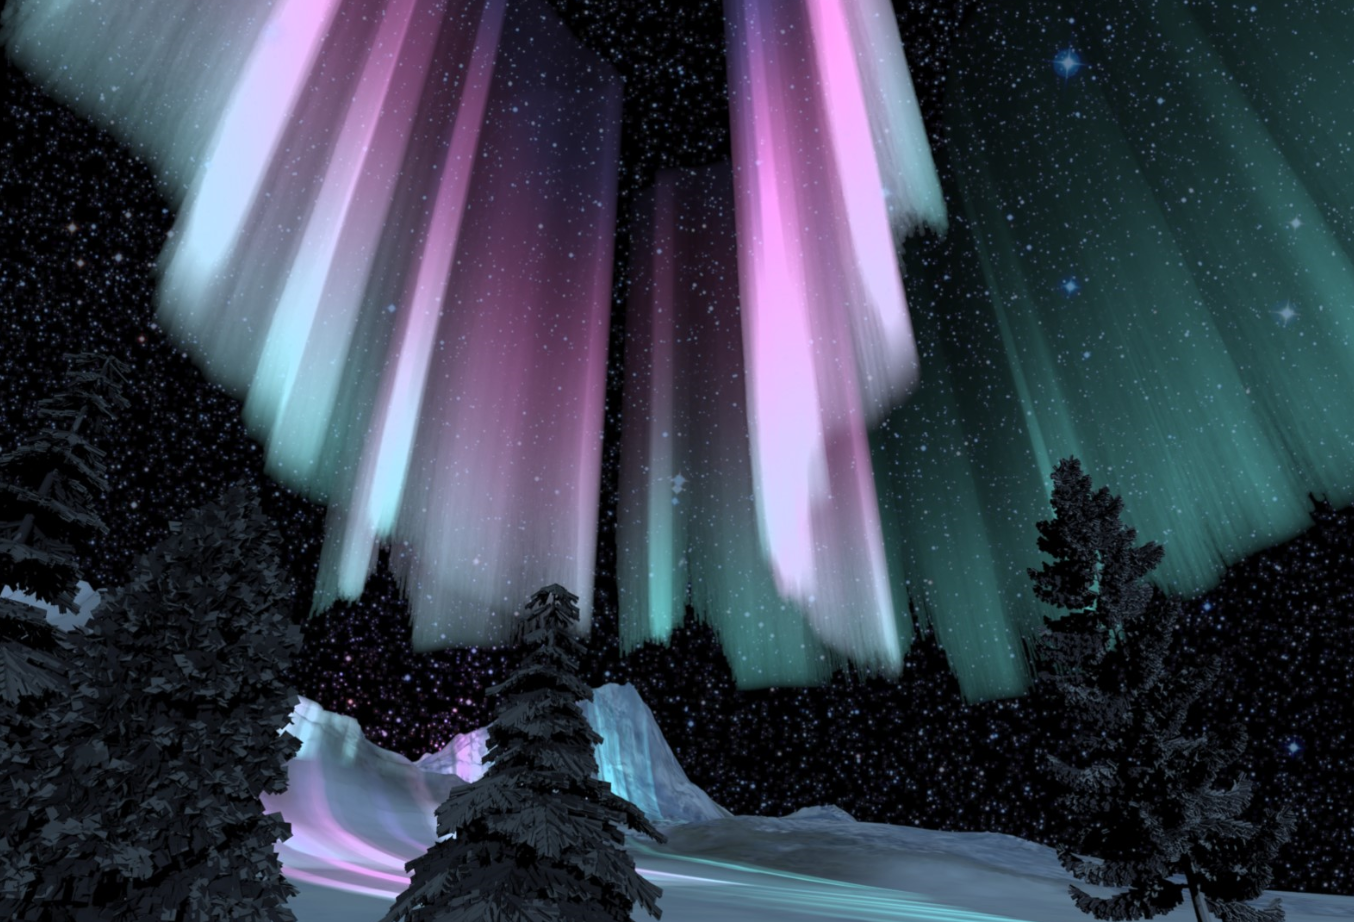
\includegraphics[width=0.95\linewidth]{./aurora}
\caption{aurora: final image}
\label{fig:aurora}
\end{figure}

\section{Conclusion}

\subsection{Challenges}

The biggest challenges in the project come from lacking of complete, physically plausible explanation about generating aurora and determining the emission light from it. The reference paper got around this problem by using rasterization instead. However, we are inclined to try rendering aurora in a more 'graphical' way, so we designed a volume grid to implement volumetric photon mapping algorithm.

Another challenge comes from tweaking the parameters in the script. It turns out to be a long and tedious work in the end, probably longer than the time we spent on coding and debugging our program!

\subsection{Division of Work}

We figured the techniqal framework for rendering aurora together. Tao Du primarily worked on volumetric photon mapping and extending the surface integrator. Wenlong Lu primarily worked on modeling the aurora, including simulating the footprint and adding multiple noises. We helped each in the process and worked together to set up the scene and the pbrt scripts for rendering the final image.  

\bibliographystyle{plain}
\bibliography{references}

\end{document}
